\subsubsection{Hodgkin-Huxleyマルチコンパートメントモデル}
\label{subsec:hh-model}
\paragraph{Hodgkin-Huxleyモデル}~\\
神経系における情報の伝達は, ニューロンの電気的な活動によって行われる.
こうしたニューロンの電気的活動を表現する方法として,
1952年にHodgkinとHuxleyによってヤリイカの神経の活動電位の研究を基にした微分方程式のモデルが考案された\cite{hh}.\\
Hodgkin-Huxleyモデルでは, 各イオンに対するニューロンの細胞膜の等価性を基に, ニューロンの電気的活動を微分方程式を用いて表現している.\\
他のモデルと比べ計算量が多い一方, 実際の生物の神経系の働きに近くたいていのイオンチャネルのモデルを表すことができるという特徴を持っている.\\

\subparagraph{モデルの定式化}~\\
\label{subpar-hh-model}
ニューロンはイオンを通さない脂質二重膜によって構成され, 特定のイオンを選択的に透過させるチャネルと呼ばれるタンパク質が膜上に分布している.
この時, 図\ref{fig:hh-circuit}に示したHodgkin-Huxleyモデルの細胞膜の等価回路のように,
神経細胞を細胞膜を容量$C_M$のキャパシタ, チャネルを透過するイオンの流れを抵抗$R_i$(コンダクタンスを用いると$R_i = \frac{1}{g_i}$と表わせる), 起電力$E_i$の電池からなる電気回路と見做すと, 膜を流れる全電流$I_M$は,
\begin{eqnarray}
  I_M & = & C_M\frac{dV}{dt} + \sum_{i} I_i\\
  I_i & = & g_i (V - E_i)\\
\end{eqnarray}
と膜電位Vに関する常微分方程式の形で表すことができる. 尚, 式中のiはイオンチャネルの種類を, $E_i$はそれぞれのイオンに特有な平衡電位を表している.\\
また, 前述した抵抗の逆数であるコンダクタンス$g_i$は
\begin{eqnarray}
  g_i(V, t) & = &\overline{g}_im(V, t)^xh(V,t)^y\\
\end{eqnarray}
と記述される.\\
\clearpage
\begin{figure}[htb]
 \begin{center}
    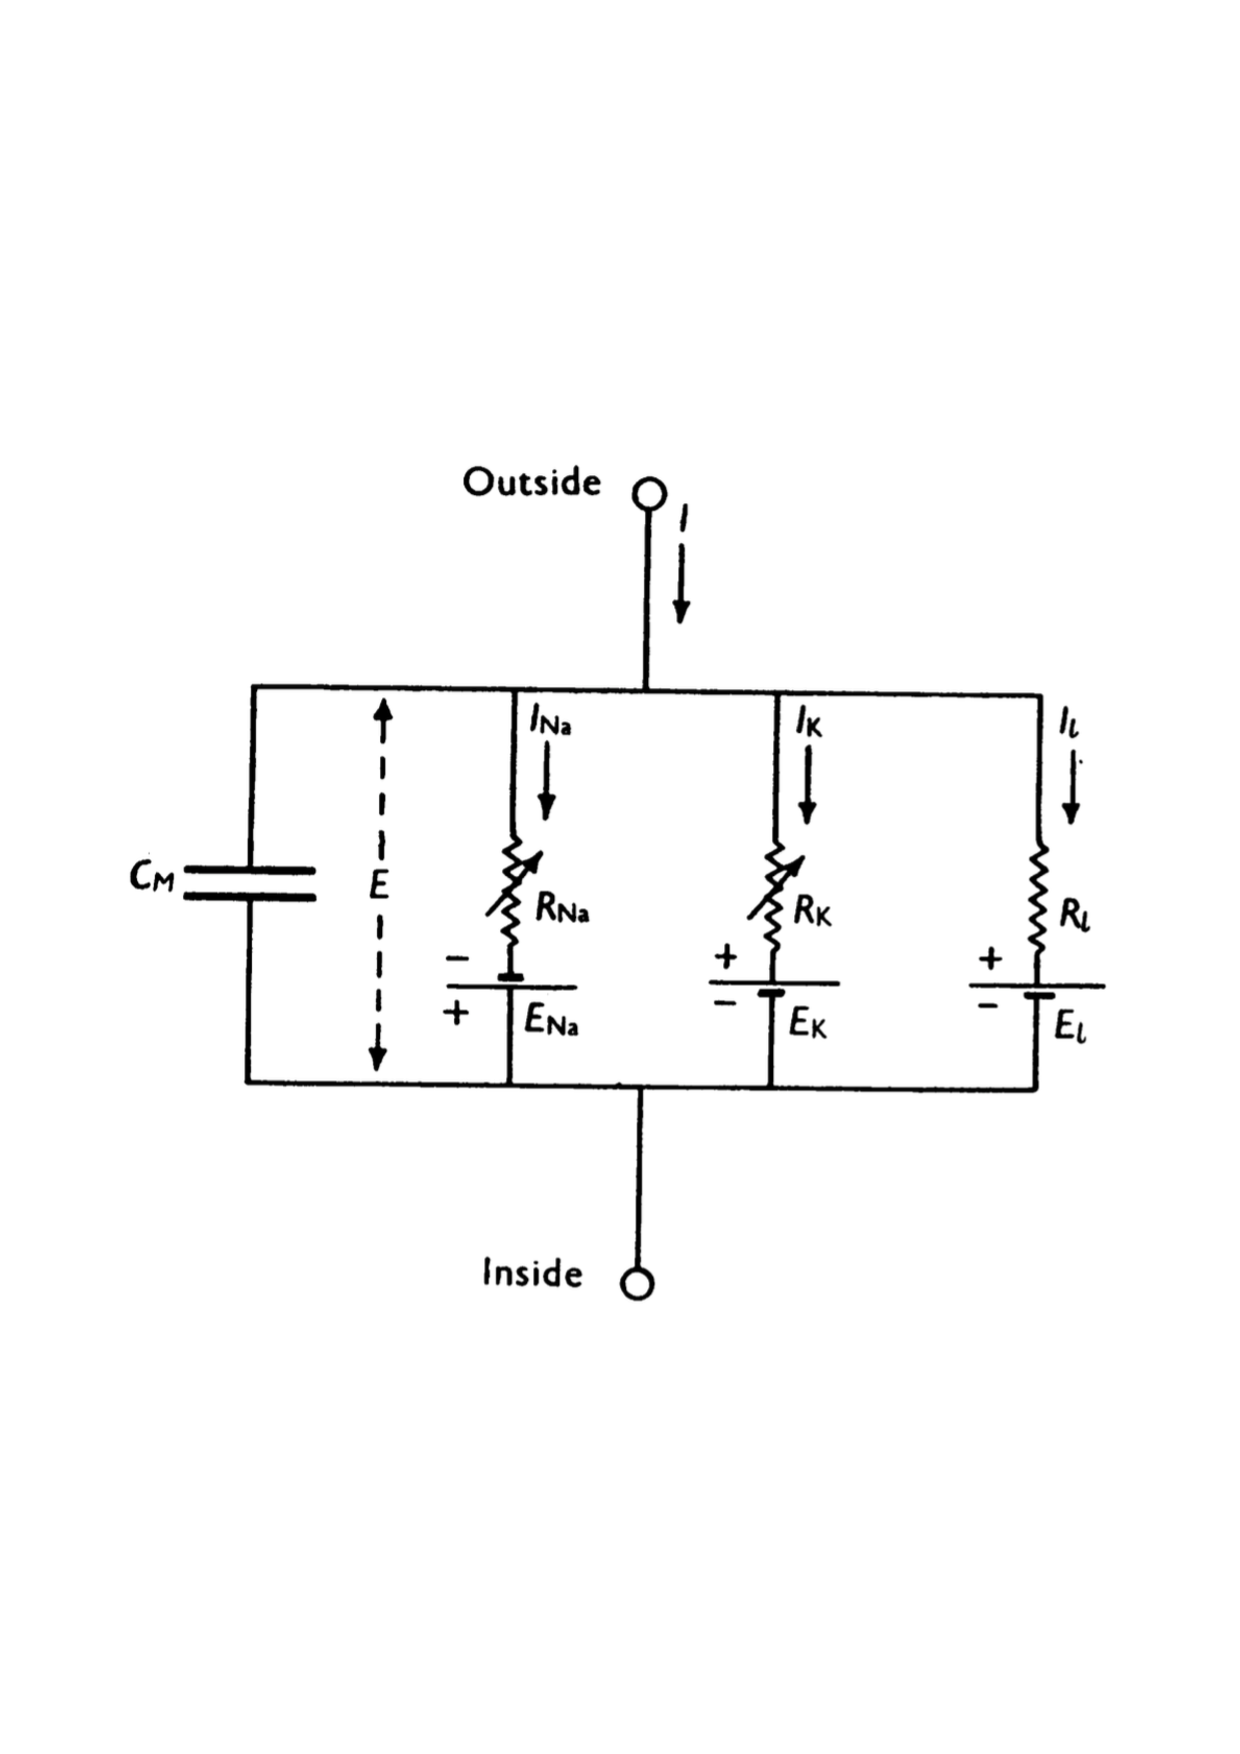
\includegraphics[width=10cm]{./images/hh-circuit.pdf}
    \caption{Hodgkin-Huxleyモデルの細胞膜の等価回路}
    \label{fig:hh-circuit}
 \end{center}
\end{figure}
\clearpage
$\overline{g}_i$は$g_i$の最大値であり, $m, h \in (0, 1)$はそれぞれ活性化パラメータ, 不活性化パラメータと呼ばれる無次元数である.\\
また, x, yはそれぞれ実験データを元に求められる整数である.\\
活性化パラメータ, 不活性化パラメータであるm, hはさらにそれぞれ次の微分方程式(式2.6から式2.12)で表現される.\\
\begin{eqnarray}
  \frac{m(V,t)}{dt} & = &\frac{m_\infty(V) - m(V, t)}{\tau_m(V)}\\
  \frac{h(V,t)}{dt} & = &\frac{h_\infty(V) - h(V, t)}{\tau_h(V)}\\
  m_\infty(V) & = & \frac{1}{1 + exp(\frac{V - \Theta_m}{k_m})}\\
  h_\infty(V) & = & \frac{1}{1 + exp(\frac{V - \Theta_h}{k_h})}\\
  \tau_m(V) & = & \tau_{m_0} + \frac{\tau_{m_1}}{exp(\frac{V - \Theta_{m_1}}{\sigma_{m_1}}) + exp(-\frac{V - \Theta_{m_2}}{\sigma_{m_2}})}\\
  \tau_h(V) & = & \tau_{h_0} + \frac{\tau_{h_1}}{exp(\frac{V - \Theta_{h_1}}{\sigma_{h_1}}) + exp(-\frac{V - \Theta_{h_2}}{\sigma_{h_2}})}\\
\end{eqnarray}
この式中のパラメータはチャネルのキネティクスに関わるパラメータであり, 実験データから算出される.\\

\subparagraph{Hodgkin-Huxleyモデルを構成する各イオンチャネル}~\\
HodgkinとHuxleyが提唱したモデルにおいて, モデルは電位依存性のNaチャネルとKチャネル,
常に開いた状態であり静止膜電位を決定するリークチャネルの3種類のチャネルから構成されていた.\\
また, 各チャネルにおける電流は次の式で表せられる.\\
\begin{eqnarray}
  I_{Na} & = & \overline{g}_{Na}m^3h(V - E_{Na})\\
  I_{K} & = & \overline{g}_{K}n^4(V - E_{K})\\
  I_{l} & =& g_l(V - E_l)\\
\end{eqnarray}

\paragraph{マルチコンパートメントモデル}~\\
\ref{subpar-hh-model}で述べたHodgkin-Huxleyモデルは細胞を一つの回路と見做してモデル化しており,
その際に細胞の形態は考慮されていない. しかしながら, 実際の細胞は複雑な形態を有しており,
細胞全体ではなく細胞の一部のみが発火するような応答を示すことが知られているため\cite{fujiwara-master},
より詳細なシミュレーションを行うためには細胞の形態についてもモデル化する必要がある.\\
そこで今回マルチコンパートメントモデルという神経細胞の3次元的な特性を表現するモデルを導入する.\\
マルチコンパートメントモデルでは, 図\ref{fig:multi-compartment}のように神経細胞の形態を多数のシリンダーの連なりとして表現する.
各シリンダをコンパートメントと呼び, 前節で示したHodgkin-Huxleyモデルの計算はコンパートメント単位で行う. すなわち,
n番目のコンパートメントの親となるコンパートメントを$n_{parent}$とし, 子となるコンパートメントをそれぞれ$n_{child_{i}}$とするとき,
マルチコンパートメントHodgkin-Huxleyモデルにおける式2.1は,
\begin{eqnarray}
  I_{m}^{n} & = & C_{m}^{n}\frac{dV}{dt} + \sum_{i} I_{i}^{n} + I^{n_{parent}, n} - \sum_{i} I^{n, n_{child_{i}}}\\
\end{eqnarray}
と表される. 尚, $I^{i, j}$はi番目のコンパートメントからj番目のコンパートメントに流れる電流を表す.

( TODO : 図の差し替え)
\begin{figure}[htb]
 \begin{center}
    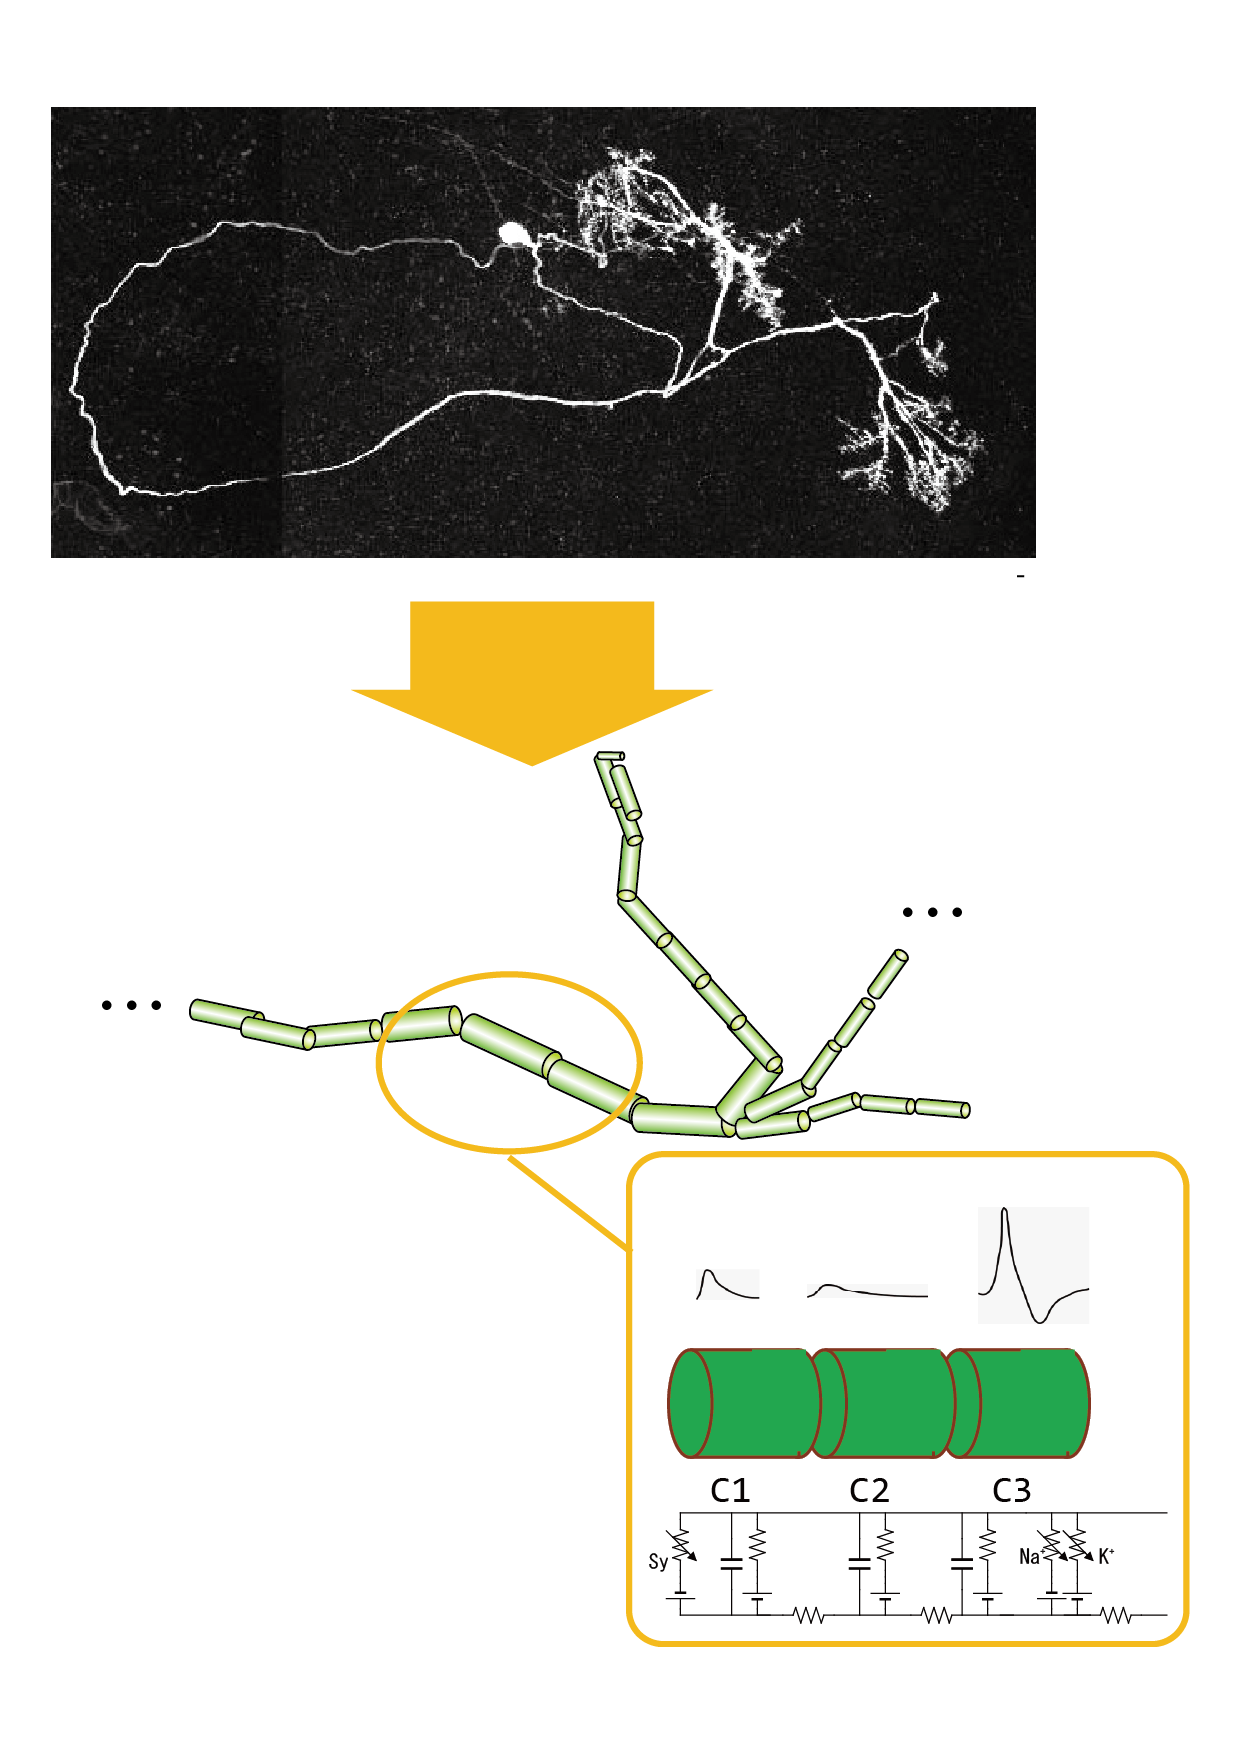
\includegraphics[width=10cm]{./images/multi-compartment.pdf}
    \caption{マルチコンパートメントモデル (Yusuke Mori. Developing implementations of the estimation of synaptic positions and the communication procedure between simulation and real environment toward whole insect brain simulation. Master's thesis, the university of Tokyo, 2014. より引用)}
    \label{fig:multi-compartment}
 \end{center}
\end{figure}
\clearpage
